% ------------------------------------------------
%          FILE:  mudanca.tex
%       CREATED:  Dom 30/Dez/2012 hs 16:00
%   LAST CHANGE:  2013 Apr 02 08:45:03 AM
%        AUTHOR:  Sérgio Luiz Araújo Silva
%          SITE:  http://vivaotux.blogspot.com
%       TWITTER:  @voyeg3r
%         SKYPE:  sergioaraujosilva
% -------------------------------------------------

\chapter{Mudança constante}

Tenha em mente que ao longo do tempo e com a sua evolução, lições que eram
difíceis se tornarão fáceis, já outras que pareciam muito difíceis se tornarão
simples, portanto colecione todos os vídeos e audios que puder. O que funciona hoje não
funcionará amanhã. Uma coisa muito importante é saber que tudo está sujeito a mudanças
esteja preparado para reconhecer quando uma mudança acontecer.
{\em leia um texto a esse respeito na seção~\ref{sec:abelha} página~\pageref{sec:abelha}}.

\noindent
Adquira o habito de ler ou ouvir dicas de outras pessoas que trilharam
o caminho da fluência no Inglês, aliás este livro é uma coleção de dicas
desse tipo. Pessoas que já trilharam o caminho falam sobre o que
funciona melhor. O aprendizado de idiomas está se tornando cada vez mais
uma atividade colaborativa, os velhos métodos estão sendo
questionados, ou seja o mundo está fervilhando de novidades, seja também
um pesquisador.

\section{Motivação e compromisso}

Será que o meu resultado final pode ser afetado pelo modo como encaro
minha atividade? \dots

\vspace{0.3\baselineskip}
\noindent
{\footnotesize \ding{42} ``Language to me is a means to and end. A tool. A vehicle that allows me
 to explore what the world has to offer. This works out great because
 my life is all about exploring and learning. Not language. Language is
 a means to an end''. \href{http://www.davidmansaray.com/language-puzzle}{David Mansaray} }

\vspace{0.3\baselineskip}
\noindent
{\footnotesize \ding{42} Find something else you’re passionate about, combine it
with language and watch your ability to learn language skyrocket. \href{http://www.davidmansaray.com/language-puzzle}{David Mansaray} }
\vspace{0.3\baselineskip}

\noindent
Tenha muito cuidado com a \emph{zona de conforto} ela é um perigo para
qualquer estudante, considere que se seu objetivo é modesto demais
sua determinação virá na mesma proporção. Sonhos pequenos, pequenas
realizações.

\subsection{Os Três pedreiros}
\label{sub:os_tr_s_pedreiros}

Uma vez um vido uma estrada, deparou-se com uma obra
em início de construção. Três pedreiros, com suas ferramentas,
trabalhavam na fundação do que parecia ser um importante projeto. O
viajante, aproximou-se curioso. Perguntou ao primeiro deles o que
estava fazendo. -- Estou sentando tijolos, respondeu
o pedreiro, o homem agradeceu dirigiu-se ao segundo pedreiro e repetiu a
pergunta.

\noindent
-- Estou construindo uma parede.  O viajante queria saber o que seria
aquela construção, agradeceu ao pedreiro e se dirigiu então ao
terceiro pedreiro: -- O que está você fazendo?

\noindent
Este respondeu: -- Estou construindo uma Catedral!

\noindent
Seguindo caminho o viajante observou que os três estavam
fazendo a mesma coisa mas o que mudava era apenas o modo
como cada um deles encarava sua atividade. Moral da história,
\emph{``O modo como encaramos a realidade determina o quão difícil ou
prazeiroso é a realização de nossas atividades''}.

\vspace{0.3\baselineskip}
\noindent
{\footnotesize \ding{42} A atitude mental é a chave para atingir
grandes resultados na vida, pois se você encara sua atividade
como um meio de atingir algo maior essa atividade torna-se prazeirosa.}

% subsection os_tr_s_pedreiros (end)

\subsection{O inglês não como um fim em si}
\label{sub:o_ingl_s_n_o_como_um_fim_em_si}

\noindent
Busque uma fonte inspiradora para estudar inglês, acho que ganhar muita grana
no futuro com a sua melhor qualificação, ter mais qualidade de vida é um bom
começo, mas saiba que se você não tiver uma motivação muito profunda você não
conseguirá manter o mesmo ritmo de estudos. Desenvolva o seu auto didatismo,
não espere soluções prontas. O estudo do inglês deve ser algo prazeiroso,
reflita positivamente acerca de suas pretensões e principalmente crie uma imagem
mental de como sua vida já está mudando e o quanto irá mudar para melhor com
suas conquistas.

\noindent
Pense no inglês como um meio de atingir um objetivo maior, afinal de
contas você estuda inglês não por ele em si, você estuda inglês para
poder viajar para fora do país, para conseguir um emprego melhor etc.

% subsection o_ingl_s_n_o_como_um_fim_em_si (end)

\vspace{0.3\baselineskip}
\noindent
{\footnotesize \ding{42} Lembre-se que o seu nível de compromisso é um dos principais
fatores que irá determinar seu sucesso.}

\vspace{0.3\baselineskip}
\noindent
{\footnotesize \ding{42} Cadastre-se em vários serviços de estudo de idiomas, assim você estará assumindo compromissos
para os quais é mais difícil arranjar desculpas, se você estuda inglês em grupo e tem reuniões periódicas isso
aumenta o seu comprometimento com seu objetivo. Busque no google ``learn english community''.}
% http://www.readability.com/articles/hte7e9hy

\subsubsection{Exemplo de compromisso}

Certa vez uma amiga minha me disse que havia deixado de fumar, ela também
disse isso para todos os familiares e amigos, um dia eu disse a ela, sabe minha amiga
se você não tivesse criado o compromisso sincero de deixar de fumar você não teria
dito para tantas pessoas que iria fazer isso, agora, mesmo que você pense em
desistir da ideia você iria ficar meio sem jeito diante de tantas pessoas, elas
lhe diriam ``Mas você não tinha dito que iria parar de fumar!!.'' Portanto crie
compromisso com suas metas, dentre as quais a de aprender inglês. Quando você
cria um compromisso sincero de realizar algo o universo conspira a seu favor.

\section{Faça do inglês parte de sua vida}\label{sec:EnglishLife}

Siga pessoas que postam frases em inglês no \href{http://www.twitter.com}{twitter} como
\index{Iramara Loiola} \href{http://www.twitter.com/iraloiola}{@iraloiola} \emph{Iramara Loiola} e outras tantas boas fontes
 de inspiração como: \href{http://www.twitter.com/InspireBookClub}{@InspireBookClub},
\href{http://www.twitter.com/RealLifeEng}{@RealLifeEng} etc. Veja por
exemplo a figura abaixo, se você tem o desejo sincero de aprender inglês será
impossível não buscar a tradução.

\begin{figure}[h!]
	\centering
	\caption{\footnotesize Estudando inglês no twitter}
		
\includegraphics[width=0.8\textwidth]{twitter}
	\index{twitter}
\end{figure}

\noindent
Outra forma de incrementar seus estudo é se cadastrar no site
\href{http://www.aprendendoingles.com.br/}{``English for
Reading''}\footnote{http://www.aprendendoingles.com.br/} que passará
a enviar-lhe uma piada em inglês diariamente, basta acessar o link acima
e colocar seu e-mail no campo indicado na base da página. {\em Veja um exemplo}:

\vspace{0.3\baselineskip}
%\hfill
\begin{minipage}[b]{.8\linewidth}

	{\scriptsize
	\noindent
	{\bf Women talk more than men }

	A husband, proving to his wife that women talk more than men, showed her
	a study which indicated that men use on the average only 15,000 words a day,
	whereas women use 30,000 words a day.

	She thought about this for awhile and then told her husband that women use
	twice as many words as men because they have to repeat everything they say.
	He said, "What?"

	\setlist[1]{itemsep=-5pt}
	\begin{itemize}
		\item husband - marido
		\item wife - esposa
		\item talk - falar
		\item show - mostrar
		\item average - média
		\item whereas - ao passo que
		\item think (think, thought, thought) - pensar
		\item awhile - por alguns instantes
		\item twice - duas vezes
	\end{itemize}
	}
\end{minipage} \hfill

\vspace{0.3\baselineskip}
Há também um site muito legal chamado
\href{http://www.tumblr.com}{``tumblr''}\footnote{www.tumblr.com} no qual tem
um canal chamado \href{http://icanread.tumblr.com/}{``i can
read''}\footnote{http://icanread.tumblr.com/} no qual são postadas muitas
frases legais em inglês como esta \dots

%\vspace{0.3\baselineskip}
\begin{figure}[h!]
	\caption{\footnotesize Uma das muitas imagens do {\bf ``i can read''}}
    \centering
		
\includegraphics[width=0.6\textwidth]{tumblr}
	\index{Tumblr}
\end{figure}

\noindent
{\footnotesize \ding{42} Outro site muito bom para praticar a leitura é o quotes love and life
 \href{http://quotesloveandlife.com/}{http://quotesloveandlife.com/} }

\noindent Se você é da área de informática por exemplo pode se cadastrar no
site \href{http://stackoverflow.com}{stackoverflow.com}\footnote{http://stackoverflow.com},
nele temos listas de discussão divididas por assunto, dessa forma você aprende
algo do seu interesse ao mesmo tempo que estuda inglês, e segundo alguns, esta
é uma das melhores formas de se aprender inglês, assim como se pode aprender
gramática sem estar estudando diretamente gramática, com o inglês é a mesma
coisa, veja a imagem abaixo do site stackoverflow.

\begin{figure}[h!]
	\caption{\footnotesize Aprendendo a programar no stackoverflow}
	\centering
		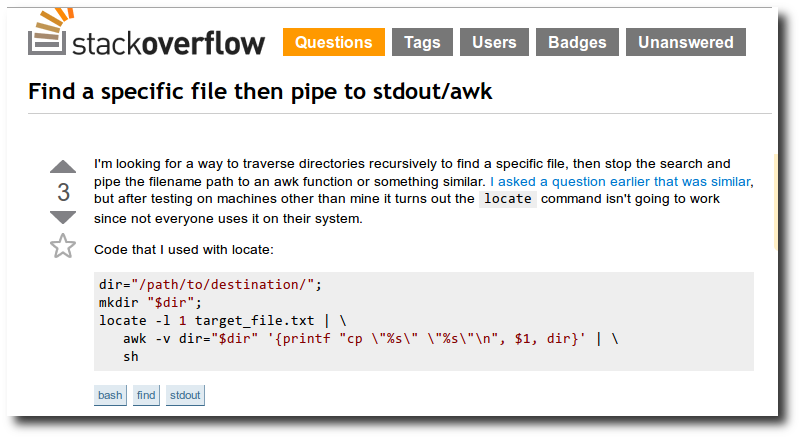
\includegraphics[width=0.8\textwidth]{stackoverflow}
	\label{img:stackoverflow}
\end{figure}

\newpage
\noindent
Configure o seu computador bem como seu smartphone para o idioma
inglês ou qualquer outro que deseje aprender, pode parecer bobagem
mas cada pequeno fragmento de inglês que você aprender faz parte de um
todo, veja um exemplo de uma mensagem do navegador chrome.

\begin{figure}[h!]
	\centering
	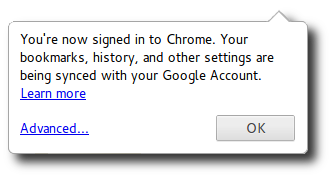
\includegraphics[width=0.8\textwidth]{chrome-browser}
	\caption{chrome-browser}
\end{figure}

\noindent \index{skype}
Um recurso que não pode deixar de ser citado é o \href{http://www.skype.com}{http://www.skype.com} mas
as pessoas tem dificuldades de encontrar parceiros de conversa, para resolver esse problema
O skype tem um link específico para pessoas interessadas em aprender outras línguas o link é este:  \\

\newpage
\href{https://community.skype.com/t5/Language-learning/bd-p/Languages}{https://community.skype.com/t5/Language-learning/bd-p/Languages}

\begin{figure}[h!]
	\centering
	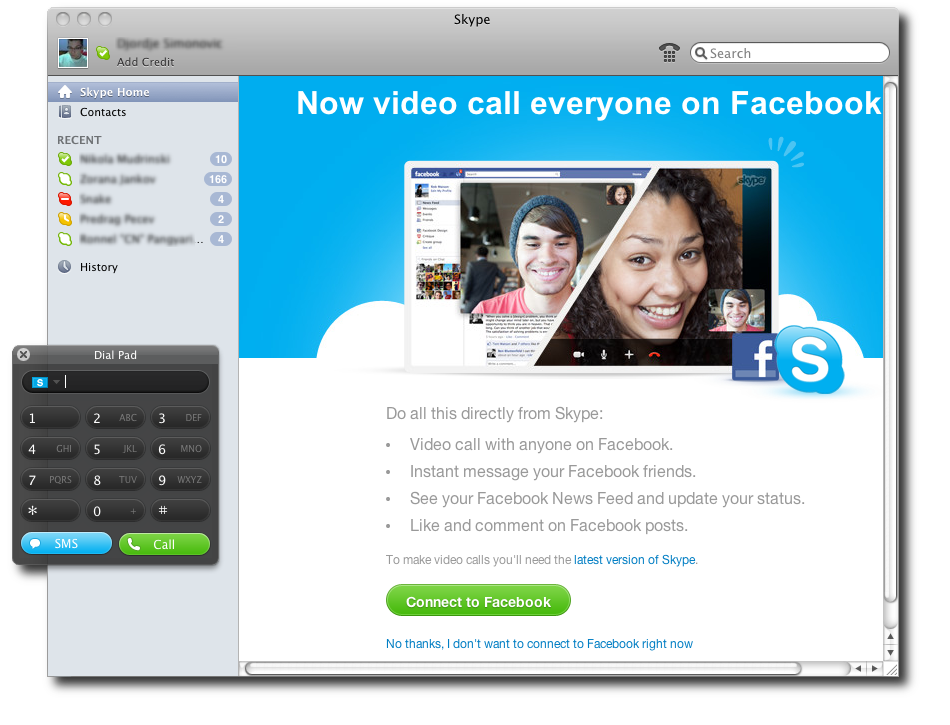
\includegraphics[width=0.8\textwidth]{skype}
	\caption{uma imagem do skype}
\end{figure}

\noindent
O site \href{https://www.verbling.com}{https://www.verbling.com} fornece um serviço parecido com o que é oferecido
pelo skype, contudo ele usa como ferramenta o serviço do google
chamado ``Google Hangouts'', você se cadastra ele pede que você
preencha qual a sua lingua de origem e qual lingua deseja aprender.
Ele oferece dois modos de estudar, um em que ele busca um parceirto da
lingua desejada que deseja aprender sua lingua, e no outro modo você
assiste e/ou entra em um Hangout existente.

\section{Aprenda a digitar}

Volta e meia você precisará de sites tradutores como
o \href{http://translate.google.com}{tradutor do
google}\footnote{http://translate.google.com/} e neles por vezes ao invés de
colar uma frase você terá que digitar, irá se cadastrar no site {\em \href{http://duolingo.com}{Duolingo}},
lá você terá muitas lições nas quais você ouve um audio e terá que digitar
o que ouviu. Outra opção possível é o site
\href{http://www.lingue.pt/}{Linguee}\footnote{http://www.linguee.pt/} no qual
digitamos uma palavra e ele nos mostra a mesma dentro de um contexto.  Se sua
digitação é ruim isso será um impecilho.

\vspace{0.3\baselineskip}
\noindent
{\footnotesize \ding{42}  Um programa livre muito bom para aprender a digitar,
é o \href{http://klavaro.sourceforge.net/pt/index.html}{klavaro}\footnote{http://klavaro.sourceforge.net/pt/index.html}.}

\section{Curso gratuito na Internet}
\index{Duolingo}

Um projeto bastante inovador no aprendizado de idiomas é o \index{Duolingo}
\href{http://duolingo.com}{Duolingo}\footnote{http://duolingo.com} a proposta
é que os usuários aprendam um idioma enquanto ajudam a traduzir artigos
e documentos. Recentemente o {\em Rubens Queiroz de Almeida}\footnote{queiroz@iname.com} o mesmo criador do
{\em livro das 1000 palavras mais comuns do inglês}\footnote{Baixe o livro aqui: http://goo.gl/jbyBZ} publicou no site
Dicas-l da Unicamp um artigo intitulado \href{http://www.dicas-l.com.br/arquivo/colaboracao\_em\_massa\_na\_internet.php}{``Colaboração
em massa na Internet''}\footnote{http://www.dicas-l.com.br/arquivo/colaboracao\_em\_massa\_na\_internet.php}
 falando sobre o projeto Duolingo ele inclusive traduziu um vídeo inteiro no qual um dos criadores
do Duolingo fala como surgiu a ideia do mesmo.

%\vspace{0.3\baselineskip}
\begin{figure}[h!]
	\centering
	\caption{Captura de tela do site {\em Duolingo}}
	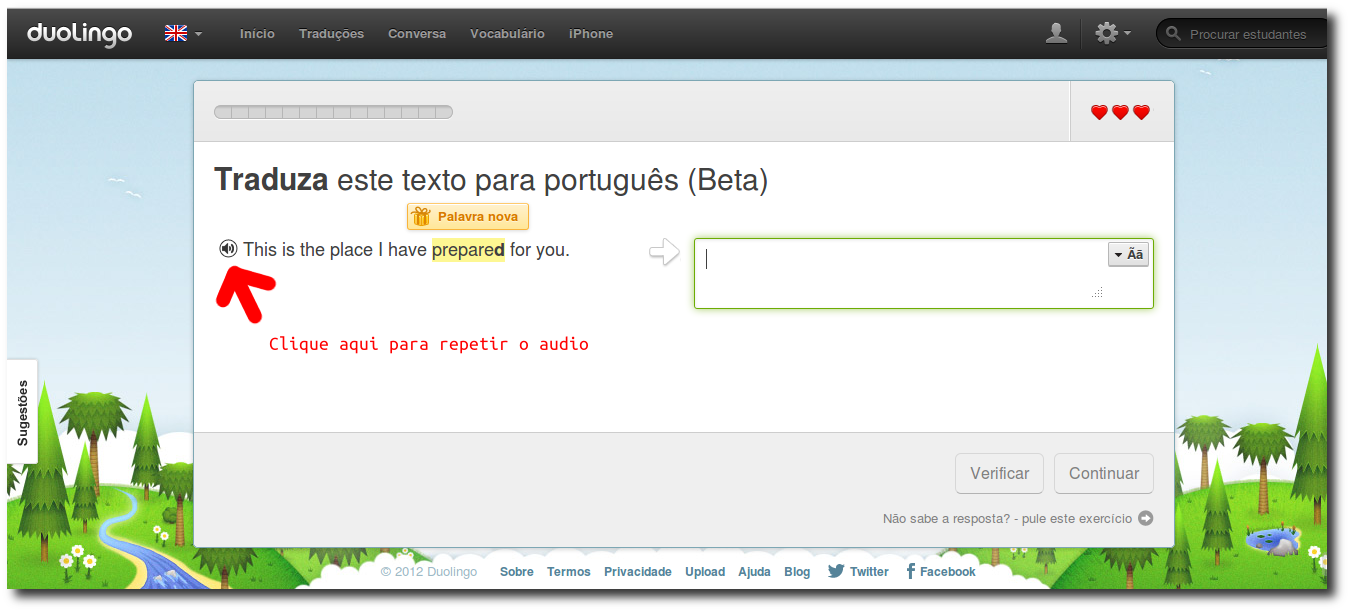
\includegraphics[width=0.8\textwidth]{duolingo} \\
\end{figure}

\begin{figure}[h!]
	\centering
	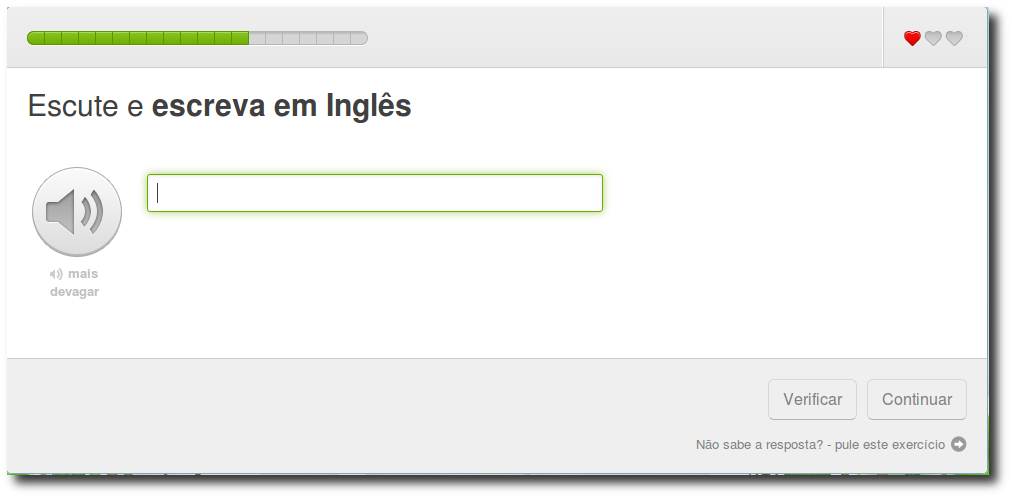
\includegraphics[width=0.8\textwidth]{duolingo-2}
\end{figure}

\vspace{0.3\baselineskip}
{\footnotesize \ding{42}  Há também uma versão do duolingo para Android\footnote{Smartphone do google}}

\section{Leia e escreva em inglês constantemente}
\label{sec:leia_e_escreva_em_ingl_s_constantemente}

Ao ler e escrever você aumentará seu vocabulário constantemente,
quando você formula novas frases vez por outra terá que buscar
palavras que ajudem na contrução de ideias. Durante a leitura proceda
a mesma em voz alta para melhorar sua pronúncia, ao mesmo tempo em que
surgirão constantemente palavras novas, marque-as e busque no site
\href{http://linguee.com}{http://linguee.com} frases contendo a
palavra em questão, anote as frases em formato de \emph{Flashcards}.
(veja mais sobre os Flashcards na
seção~\ref{sub:programas_para_memoria_o}
página\pageref{sub:programas_para_memoria_o})  São retângulos em
cartolina em que de um lado está a frase em inglês e do outro a sua
tradução.

Existe um site chamado \href{http://lang-8.com/}{http://lang-8.com/}
no qual os textos que você envia serão corrigidos por nativos da
lingua alvo e você poderá ajudar pessoas que desejam aprender
português, assim você controi aos poucos um círculo de amizades em que
a ajuda mútua é a tônica.

% section leia_e_escreva_em_ingl_s_constantemente (end)

\section{Crie um livro de anotações}\label{sec:evernote}
\index{Evernote}

Crie um livro de anotações no qual você anota frases nas quais aparecem
palavras novas, isto é necessário pelo fato de que novas palavras se não
anotadas são dificilmente memorizadas, a revisão periódica das anotações
garante o aprendizado. Outra possibilidade é criar uma conta no site
\href{https://evernote.com/}{evernote}\footnote{https://evernote.com/} no qual
você pode salvar artigos inteiros para consultas posteriores. A grande vantagem
de ter uma espécie de bloco de notas online é que independente de onde você
esteja, seja em casa, no trabalho ou durante uma viagem o seu conteúdo está
acessível.  Também fortemente recomendado é a criação de uma conta no site de
favoritos online
\href{https://www.delicious.com/}{delicious}\footnote{https://www.delicious.com/}.
Normalmente as pessoas usam os favoritos do navegador, contudo as páginas que
você salva estão geralmente no computador de casa, quando você chega no
trabalho os favoritos de casa não estão mais acessíveis e vice-versa, com
o {\em delicious} seus favoritos estão em qualquer lugar em que exista acesso
a web.

\vspace{0.3\baselineskip}
\noindent
{\footnotesize \ding{42}  Há uma versão do {\em evernote} para {\em Android}}

\vspace{0.3\baselineskip}
\noindent
{\footnotesize \ding{42} There is no growth without change, no change without fear or loss, and no loss
without pain. http://simurl.com/zobbaj  pg 220 }

\vspace{0.3\baselineskip}
\noindent
{\footnotesize \ding{42} this section brings to you one gift :) \href{http://www.ecenglish.com/learnenglish/}{http://www.ecenglish.com/learnenglish/} }

